% !TEX root = thesis.tex
\documentclass[12pt,a4paper,titlepage,listof=totoc,bibliography=totoc,chapteratlists=0pt]{scrreprt}
\input{global-const.tex}
\input{header}

% -----------------------------------------------
% PAKETE – müssen VOR \begin{document} stehen!
% -----------------------------------------------
\usepackage{listings}
\usepackage{xcolor}

\lstset{
    basicstyle=\ttfamily\small,
    keywordstyle=\color{blue},
    stringstyle=\color{orange},
    commentstyle=\color{gray},
    showstringspaces=false,
    breaklines=true,
    frame=single,
    backgroundcolor=\color{gray!10}
}

\makeatletter
\def\bstctlcite{\@ifnextchar[{\@bstctlcite}{\@bstctlcite[@auxout]}}
\def\@bstctlcite[#1]#2{\@bsphack
    \@for\@citeb:=#2\do{%
        \edef\@citeb{\expandafter\@firstofone\@citeb}%
        \if@filesw\immediate\write\csname #1\endcsname{\string\citation{\@citeb}}\fi}%
    \@esphack}
\makeatother
\clubpenalty=10000 
\widowpenalty=10000
\displaywidowpenalty=10000
\interfootnotelinepenalty=10000
\title{\thesistitle}
\makeatletter
\@ifundefined{fourthauthor}{
  \@ifundefined{thirdauthor}{
    \author{\firstauthor, \secondauthor}
  }{
    \author{\firstauthor, \secondauthor, \thirdauthor}
  }
}{
  \author{\firstauthor, \secondauthor, \thirdauthor, \fourthauthor}
}
\makeatother
\makeindex
\makeglossaries

\begin{document}

\bstctlcite{IEEEexample:BSTcontrol}
\newcommand{\reminder}[1]
{ \textcolor{red}{<[{\bf\marginpar{\mbox{$<==$}} #1 }]>} }
\newcommand{\icode}[1]{\lstinline$#1$}
\setstretch{1.433}
\renewcommand{\arraystretch}{1.2}
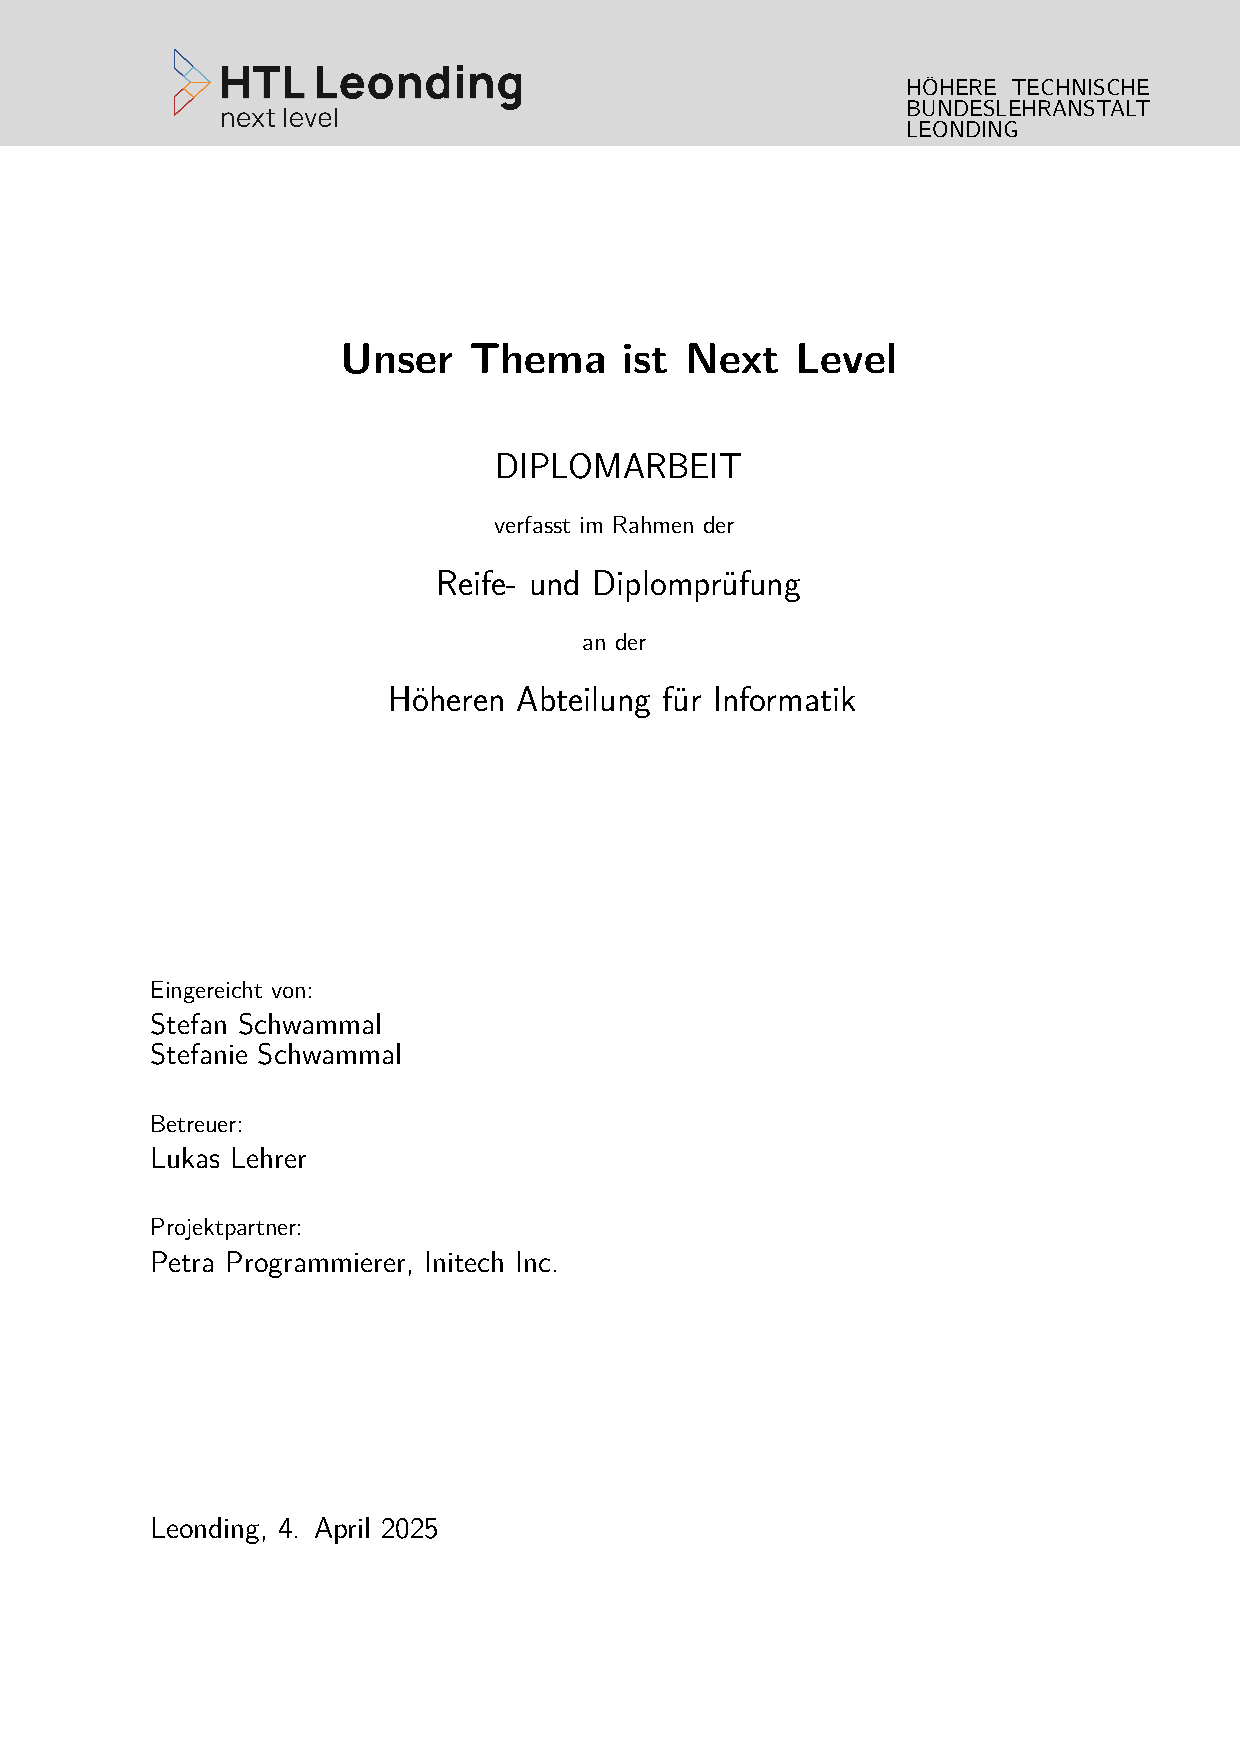
\includepdf{./titlepage/coversheet}
\pagenumbering{Roman}
\newpage
\input{oath}
\input{./sections/abstract}
\pagestyle{plain}
\IfStrEq{\thesislang}{de}
{
    \renewcommand{\lstlistlistingname}{Quellcodeverzeichnis}
}
{
 % keep at list of listing
}
\tableofcontents
\newpage
\setcounter{RPages}{\value{page}}
\setcounter{page}{0}
\pagenumbering{arabic}
\pagestyle{scrheadings}

\begin{spacing}{1}
\chapter{Einleitung}\label{chapter:introduction}
\end{spacing}
\setauthor{Markus Tran}
\section{Motivation und Problemstellung der Abo-Verwaltung}

Die zunehmende Verbreitung von Streaming-Diensten hat dazu geführt, dass viele Nutzer gleichzeitig mehrere Abonnements unterhalten. Dabei entsteht ein Problem, das in der Praxis häufig übersehen wird: Verschiedene Anbieter, wie etwa Netflix und Disney+, stellen teilweise identische Inhalte zur Verfügung. Dennoch werden beide Dienste parallel abonniert und abgerechnet, obwohl ein einziges Abonnement für den Zugriff auf den gewünschten Inhalt ausreichen würde. Dies führt zu unnötigen, wiederkehrenden Kosten für den Endnutzer.
Darüber hinaus fehlt es vielen Nutzern an einer zentralen Übersicht über ihre bestehenden Abonnements, was die bewusste Entscheidung für oder gegen einen bestimmten Anbieter erheblich erschwert. Die vorliegende Diplomarbeit greift diese Problemstellung auf und entwickelt eine Lösung, die Nutzern ermöglicht, fundierte Entscheidungen darüber zu treffen, welche Abonnements für sie tatsächlich einen Mehrwert bieten und welche gekündigt werden können.

\section{Zielsetzung der Diplomarbeit}
Ziel dieser Diplomarbeit ist die Konzeption und Entwicklung einer webbasierten Plattform zur zentralen Verwaltung von Streaming-Abonnements. Die Anwendung soll Nutzern ermöglichen, alle ihre aktiven Streaming-Dienste an einem einzigen Ort zu bündeln und jederzeit einen strukturierten Überblick über ihre Abonnements zu behalten.
Ein weiteres zentrales Ziel ist die gezielte Unterstützung bei der Inhaltssuche: Sucht ein Nutzer nach einem bestimmten Film oder einer Serie, soll die Plattform transparent anzeigen, bei welchen seiner bereits abonnierten Anbieter dieser Inhalt verfügbar ist. Damit wird nicht nur der Suchaufwand minimiert, sondern auch die Grundlage für eine bewusstere und kosteneffizientere Nutzung von Streaming-Diensten geschaffen.

\section{Nutzen der Anwendung für Endanwender}
Der unmittelbare Nutzen der entwickelten Anwendung für Endanwender liegt in der deutlichen Reduktion von Verwaltungsaufwand und unnötigen Ausgaben. Durch eine übersichtliche und intuitiv bedienbare Benutzeroberfläche erhalten Nutzer auf einen Blick eine vollständige Darstellung ihrer aktiven Abonnements sowie deren Kosten.
Zusätzlich profitieren Nutzer von einer intelligenten Inhaltssuche, die vorhandene Abonnements berücksichtigt und den günstigsten bzw. bereits bezahlten Anbieter für einen gesuchten Inhalt hervorhebt. Insgesamt trägt die Anwendung dazu bei, das Management mehrerer Streaming-Dienste erheblich zu vereinfachen und die finanzielle Transparenz für den Nutzer zu erhöhen.

\section{Aufbau der Diplomarbeit}
Die vorliegende Arbeit gliedert sich in mehrere thematische Abschnitte. Nach der Einleitung und der Analyse der Ausgangssituation werden die technischen Grundlagen und die eingesetzten Technologien vorgestellt.
Die Implementierung basiert auf einem modernen Technologie-Stack: Als Backend-Framework wird Quarkus eingesetzt, während das Frontend mit Angular realisiert wird. Für die Authentifizierung und das Identitätsmanagement kommt Keycloak als externe Bibliothek zum Einsatz. Die Bereitstellung von Film- und Seriendaten erfolgt über die The Movie Database (TMDb) API, während eine relationale Datenbank die persistente Speicherung und Verwaltung der Nutzerdaten übernimmt.
Abschließend werden die Ergebnisse evaluiert sowie ein Ausblick auf mögliche Weiterentwicklungen gegeben.

\begin{spacing}{1}
\chapter{Ausgangssituation und Analyse}\label{chapter:currentSituation}
\end{spacing}
\section{Aktuelle Herausforderungen bei Streaming-Abonnements}
Der Streaming-Markt hat sich in den vergangenen Jahren stark fragmentiert. Inhalte, 
die früher auf einer einzelnen Plattform verfügbar waren, sind heute auf zahlreiche Anbieter 
verteilt. Für Endnutzer entsteht dadurch die Notwendigkeit, mehrere Abonnements gleichzeitig 
zu verwalten, um Zugang zu einem breiten Inhaltsspektrum zu erhalten. Gleichzeitig führt die 
fehlende Transparenz darüber, welcher Inhalt auf welcher Plattform verfügbar ist, dazu, 
dass Nutzer denselben Inhalt unter Umständen mehrfach bezahlen, ohne sich dessen bewusst zu sein.
\section{Probleme durch parallele Abos und doppelte Abbuchungen}
Ein zentrales Problem bei der parallelen Nutzung mehrerer Streaming-Dienste ist 
der finanzielle Mehraufwand durch redundante Abonnements. Da viele Anbieter überlappende 
Inhaltsbibliotheken aufweisen, kommt es häufig vor, dass ein Film oder eine Serie 
bei mehreren Diensten gleichzeitig verfügbar ist, die der Nutzer bereits abonniert hat. 
Mangels einer zentralen Übersicht bleibt dieser Umstand oft unentdeckt, was zu vermeidbaren 
monatlichen Mehrkosten führt.Darüber hinaus 
veranlasst die unklare Verfügbarkeit von Inhalten Nutzer dazu, bei jeder Suchanfrage mehrere Plattformen manuell zu durchsuchen. Eine konsolidierte Plattform, die diese Informationen bündelt, kann diesen Aufwand erheblich reduzieren.
\section{Bestehende Lösungen und deren Schwächen}
Es existieren bereits Plattformen, die für einen gesuchten Film oder eine Serie anzeigen, auf welchen Streaming-Diensten dieser Inhalt verfügbar ist. Ein bekanntes Beispiel hierfür ist JustWatch. Diese Lösungen bieten jedoch keine Funktionalität zur Verwaltung eigener Abonnements und beschränken sich in der Regel auf die Darstellung populärer Inhalte und Anbieter. Zudem ähneln diese Plattformen eher Bewertungs- und Entdeckungsportalen als einem persönlichen Abonnement-Management-Tool. Eine individualisierte Übersicht, die die tatsächlich vom Nutzer abonnierten Dienste in den Mittelpunkt stellt, wird von bestehenden Lösungen nicht geboten.
\section{Abgrenzung zu Standard-Webprojekten}
Im Unterschied zu herkömmlichen Webprojekten zeichnet sich die vorliegende Anwendung durch mehrere technische und konzeptionelle Besonderheiten aus.
Ein wesentliches Merkmal ist der Einsatz von Keycloak als externes Identity- und Access-Management-System. Anstatt eine eigene Authentifizierungslösung zu implementieren, wird die Nutzerverwaltung, inklusive Registrierung, Login und Rechtevergabe, vollständig an Keycloak ausgelagert. Dies erhöht die Sicherheit der Anwendung erheblich und entspricht modernen Standards im Bereich der Authentifizierung.
Eine weitere Besonderheit liegt in der gezielten Nutzung der The Movie Database (TMDb) API zur Bereitstellung von Film- und Seriendaten. Durch diese Auslagerung auf eine externe, kontinuierlich gepflegte Datenquelle wird der eigene Datenspeicher auf ein Minimum reduziert. Gleichzeitig wird sichergestellt, dass Nutzer stets auf aktuelle und vollständige Inhaltsinformationen zugreifen können, ohne dass eine aufwändige eigene Datenpflege notwendig wäre.
Die Kombination aus externem Identitätsmanagement, API-basierter Datenbeschaffung und einer personalisierten Abonnementverwaltung hebt dieses Projekt deutlich von einem klassischen CRUD-Webprojekt ab und stellt erhöhte Anforderungen an die Systemarchitektur, die Schnittstellenintegration sowie die Datensicherheit.


\begin{spacing}{1}
\chapter{Fachlicher Hintergrund: Abo- und Mediatheken-Management}\label{chapter:currentSituation}
\end{spacing}
\setauthor{Markus Tran}
Die vorliegende Anwendung adressiert ein konkretes Problem des modernen
Medienkonsums: die zunehmende Unübersichtlichkeit bei der Verwaltung mehrerer
paralleler Streaming-Abonnements. Um die Relevanz und den Mehrwert der
entwickelten Lösung zu verdeutlichen, werden in diesem Kapitel die fachlichen
Grundlagen des Abo- und Mediatheken-Managements erläutert.


\section{Zentrale Verwaltung von Abonnements und Laufzeiten}

Der Markt für Video-on-Demand-Dienste hat sich in den vergangenen Jahren stark
ausdifferenziert. Neben den frühen Marktführern wie Netflix und Amazon Prime
Video sind zahlreiche weitere Anbieter entstanden -- darunter Disney+, Apple TV+,
Paramount+ und viele nationale Mediatheken. Eine repräsentative Studie des
Digitalverbands Bitkom aus dem Jahr 2023 zeigt, dass ein Großteil der deutschen
Haushalte gleichzeitig mehrere Streaming-Dienste abonniert hat.

Diese Fragmentierung des Angebots führt zu einer praktischen Herausforderung:
Nutzerinnen und Nutzer verlieren den Überblick über ihre aktiven Abonnements,
die jeweiligen Abrechnungszeitpunkte und die damit verbundenen monatlichen oder
jährlichen Kosten. Anders als bei klassischen Dauerschuldverhältnissen -- etwa
Mobilfunkverträgen -- erfolgt die Abrechnung von Streaming-Diensten häufig
automatisch und ohne gesonderte Zahlungsbenachrichtigung, was eine unbewusste
Fortsetzung nicht mehr genutzter Abonnements begünstigt.

Eine zentrale Verwaltung von Abonnements und deren Laufzeiten schafft hier
Abhilfe. Durch die strukturierte Erfassung aller aktiven Dienste, ihrer
Abrechnungszyklen -- monatlich oder jährlich -- sowie der jeweiligen
Abrechnungsdaten erhalten Nutzer einen konsolidierten Überblick über ihre
laufenden Verpflichtungen. Dies ermöglicht eine bewusste Entscheidung darüber,
welche Dienste tatsächlich genutzt werden und welche gekündigt werden könnten.


\section{Darstellung von Verfügbarkeiten von Filmen und Serien}

Ein weiteres zentrales Problem des fragmentierten Streaming-Markts ist die
uneinheitliche Verfügbarkeit von Inhalten. Ein Film oder eine Serie ist
selten auf allen Plattformen gleichzeitig verfügbar. Stattdessen sind Inhalte
exklusiv an bestimmte Anbieter gebunden oder wechseln im Laufe der Zeit
zwischen verschiedenen Plattformen.

Für Nutzer bedeutet dies, dass die Suche nach einem konkreten Titel häufig
mehrere manuelle Suchanfragen auf unterschiedlichen Plattformen erfordert.
Dieser Prozess ist zeitaufwändig und frustrierend, insbesondere wenn der
gesuchte Inhalt auf keiner der abonnierten Plattformen verfügbar ist.

Eine Anwendung, die Filminformationen mit der Verfügbarkeit bei
Streaming-Anbietern verknüpft, löst dieses Problem. Nutzer können direkt
bei der Filmsuche erkennen, auf welchen Plattformen ein Titel verfügbar
ist und -- in Kombination mit der Abonnementverwaltung -- ob dieser Titel
auf einer ihrer bereits abonnierten Plattformen abrufbar ist. Diese
Verknüpfung von Inhaltsdaten und Abonnementstatus stellt den zentralen
fachlichen Mehrwert der vorliegenden Anwendung dar.

Die technische Grundlage für diese Funktionalität bildet die TMDB API,
die neben umfangreichen Filmdaten auch länderspezifische Informationen
zu Streaming-Verfügbarkeiten bereitstellt. Dabei wird zwischen
verschiedenen Bezugsmodellen unterschieden: Flatrate-Verfügbarkeit
im Rahmen eines Abonnements, Leihmodelle sowie Kaufoptionen. Im Kontext
der vorliegenden Anwendung sind ausschließlich Flatrate-Angebote relevant,
da der Fokus auf der Verwaltung aktiver Abonnements liegt.


\section{Mehrwert einer zentralen Applikation für Nutzer}

Der Mehrwert der entwickelten Anwendung ergibt sich aus der Zusammenführung
zweier bisher getrennter Informationsquellen: der persönlichen
Abonnementverwaltung und der Suche nach Streaming-Verfügbarkeiten. Bestehende
Lösungen adressieren diese Bereiche typischerweise isoliert voneinander.

Allgemeine Budgetverwaltungs-Apps ermöglichen die Erfassung von
Abonnementkosten, bieten jedoch keine Verknüpfung mit konkreten Filminhalten.
Streaming-Suchmaschinen wie JustWatch zeigen an, auf welchen Plattformen ein
Film verfügbar ist, verfügen jedoch über keine persönliche
Abonnementverwaltung, die den individuellen Nutzerstatus berücksichtigt.

Die vorliegende Anwendung kombiniert beide Aspekte in einer einheitlichen
Oberfläche. Nutzer können ihre Abonnements verwalten, nach Filmen suchen
und direkt erkennen, ob ein gesuchter Titel auf einer ihrer abonnierten
Plattformen verfügbar ist. Dieser personalisierte Ansatz reduziert den
kognitiven Aufwand bei Entscheidungen über Streaming-Inhalte und schafft
einen konkreten praktischen Nutzen im Alltag.

Darüber hinaus trägt die Anwendung zur Kostentransparenz bei. Durch die
strukturierte Erfassung von Abrechnungszyklen und -daten können Nutzer
ihre monatlichen Ausgaben für Streaming-Dienste besser nachvollziehen
und bewusster gestalten. Gerade bei jährlichen Abrechnungsmodellen, die
aufgrund ihres günstigeren Preises häufig gewählt werden, geht das
konkrete Abrechnungsdatum im Alltag leicht verloren.


\section{Datenschutz- und Sicherheitsanforderungen}

Da die vorliegende Anwendung personenbezogene Daten verarbeitet --
insbesondere Informationen über abonnierte Streaming-Dienste und deren
Abrechnungsdaten -- sind Datenschutz- und Sicherheitsanforderungen ein
wesentlicher Bestandteil des Systemdesigns.

Im Sinne der Datensparsamkeit, einem Grundprinzip der Datenschutz-Grundverordnung
(DSGVO), werden ausschließlich jene Daten erfasst und gespeichert, die für
die Kernfunktionalität der Anwendung erforderlich sind. Auf die Speicherung
besonders sensibler Daten wie Zahlungsinformationen oder Zugangsdaten zu
den jeweiligen Streaming-Plattformen wird bewusst verzichtet. Die Anwendung
beschränkt sich auf die Verwaltung von Metadaten der Abonnements --
Anbieter, Abrechnungszyklus und Datum der letzten Abbuchung.

Die Authentifizierung und Autorisierung der Nutzer wird vollständig über
Keycloak abgewickelt, ein etabliertes Open-Source-System für
Identity- und Access-Management. Durch diese Auslagerung wird das Risiko
einer unsicheren Eigenimplementierung von Passwortlogik eliminiert.
Zugangsdaten werden zu keinem Zeitpunkt durch die Anwendung selbst
verarbeitet oder gespeichert.

Der Zugriff auf benutzerspezifische Daten ist durch eine
rollenbasierte Zugriffskontrolle abgesichert. Geschützte Endpunkte des
Backends sind ausschließlich für authentifizierte Nutzer mit den
entsprechenden Rollen zugänglich. Das Frontend steuert darüber hinaus
den Zugriff auf geschützte Navigationsbereiche, sodass persönliche
Inhalte nicht ohne gültige Anmeldung angezeigt werden. Die Kommunikation
zwischen Frontend, Backend und Keycloak erfolgt ausschließlich über
verschlüsselte HTTPS-Verbindungen.


\begin{spacing}{1}
\chapter{Quarkus}\label{chapter:quarkus}     % <-- label geändert
\end{spacing}

\lstdefinelanguage{json}{
    basicstyle=\ttfamily\small,
    showstringspaces=false,
    breaklines=true,
    frame=single,
    backgroundcolor=\color{gray!10}
}

\lstset{
    language=java,
    basicstyle=\ttfamily\small,
    keywordstyle=\color{blue},
    stringstyle=\color{orange},
    commentstyle=\color{gray},
    showstringspaces=false,
    breaklines=true,
    frame=single,
    backgroundcolor=\color{gray!10}
}

\section{Quarkus – Grundlagen und Einsatz in der Anwendung}
\setauthor{Markus Tran}

Quarkus ist ein modernes, quelloffenes Java-Framework, das speziell für den Einsatz 
in containerisierten und Cloud-nativen Umgebungen entwickelt wurde. Ziel des Frameworks 
ist es, den Prozess der Bereitstellung von Java-Applikationen in Cloud-Umgebungen zu 
vereinfachen und zu optimieren. Dabei unterstützt Quarkus Entwicklerinnen und Entwickler 
dabei, Applikationen auch ohne tiefgehende Kenntnisse der zugrundeliegenden Infrastruktur 
bereitzustellen.

Ein wesentliches Merkmal von Quarkus ist seine Kompatibilität mit einer Vielzahl 
etablierter Frameworks und Standards. Dazu zählen unter anderem Eclipse MicroProfile, 
RESTEasy (JAX-RS), Hibernate ORM (JPA), Apache Kafka sowie Spring. Diese breite 
Unterstützung ermöglicht es, bestehende Kenntnisse und Bibliotheken direkt einzusetzen, 
ohne grundlegende Umstrukturierungen vornehmen zu müssen.

Quarkus hebt sich durch seine Leichtgewichtigkeit von anderen Java-Frameworks ab. 
Konkret äußert sich dies in einer geringen Startzeit, einem niedrigen Speicherverbrauch 
sowie der einfachen Möglichkeit, Projekte in Cloud-Umgebungen bereitzustellen.


\section{Grundprinzip von Quarkus}
\setauthor{Markus Tran}

Ein zentrales Merkmal von Quarkus liegt in der Art, wie Java-Anwendungen kompiliert 
und ausgeführt werden. Um dies zu verstehen, ist es notwendig, die zwei grundlegenden 
Kompilierungsansätze zu unterscheiden: die Just-In-Time-Kompilierung (JIT) und die 
Ahead-of-Time-Kompilierung (AOT).

\subsection{Just-In-Time-Kompilierung (JIT)}

Im klassischen Java-Ausführungsmodell wird Quellcode zunächst vom Java-Compiler in 
plattformunabhängigen Bytecode übersetzt. Dieser Bytecode wird anschließend von der 
Java Virtual Machine (JVM) interpretiert. Die JIT-Kompilierung ist dabei ein 
Optimierungsmechanismus der JVM: Häufig ausgeführte Codeabschnitte werden zur Laufzeit 
in nativen Maschinencode übersetzt, was die Ausführungsgeschwindigkeit erhöht.

Der Nachteil dieses Ansatzes liegt darin, dass die JVM beim Start der Applikation 
zunächst hochgefahren werden muss und die JIT-Optimierungen erst schrittweise während 
der Laufzeit greifen. Dies führt zu längeren Startzeiten und einem erhöhten 
Speicherverbrauch – Faktoren, die in containerisierten Umgebungen mit häufigen 
Neustarts besonders nachteilig sind.

\subsection{Ahead-of-Time-Kompilierung (AOT)}

Die Ahead-of-Time-Kompilierung verfolgt einen grundlegend anderen Ansatz: Der gesamte 
Anwendungscode wird bereits vor der Ausführung, also zum Zeitpunkt des Build-Prozesses, 
in nativen Maschinencode übersetzt. Quarkus nutzt hierfür GraalVM Native Image, ein 
Werkzeug, das Java-Anwendungen in plattformspezifische, ausführbare Binärdateien 
kompiliert.

Das Ergebnis ist eine native ausführbare Datei, die ohne eine laufende JVM auskommt. 
Dies hat folgende Vorteile:

\begin{itemize}
    \item \textbf{Schnelle Startzeit:} Da keine JVM initialisiert werden muss und alle 
    Optimierungen bereits zur Build-Zeit vorgenommen wurden, startet die Anwendung 
    in Millisekunden.
    \item \textbf{Geringer Speicherverbrauch:} Der Wegfall der JVM-Laufzeitumgebung 
    reduziert den RAM-Bedarf erheblich.
    \item \textbf{Eignung für containerisierte Umgebungen:} Kurze Startzeiten und 
    geringer Ressourcenverbrauch machen AOT-kompilierte Anwendungen besonders 
    geeignet für Kubernetes und ähnliche Plattformen.
\end{itemize}

Als Nachteil ist die deutlich längere Build-Zeit im Vergleich zur JIT-Kompilierung 
zu nennen, da die gesamte Kompilierung und Optimierung vorab stattfindet.

\subsection{Hot Reload}

Für den Entwicklungsprozess bietet Quarkus einen sogenannten Hot-Reload-Mechanismus, 
bekannt als \textit{Quarkus Dev Mode}. Dabei werden Änderungen am Quellcode automatisch 
erkannt und ohne Neustart der Anwendung übernommen. Dies beschleunigt den 
Entwicklungszyklus erheblich, da zeitaufwändige Neustarts entfallen. Der Dev Mode 
verwendet intern JIT-Kompilierung, um diese schnelle Rückkopplungsschleife zu 
ermöglichen – die AOT-Kompilierung wird lediglich für den finalen Build eingesetzt.


\section{Quarkus in der vorliegenden Applikation}
\setauthor{Markus Tran}

Quarkus wird in der vorliegenden Anwendung als Hauptframework für das Backend verwendet. 
Für die Datenbankanbindung kommt Hibernate ORM mit Panache zum Einsatz, das eine 
vereinfachte Abstraktion des JPA-Standards bietet und den Datenbankzugriff mit weniger 
Boilerplate-Code ermöglicht.

Die Anwendung wird mittels AOT-Kompilierung als native ausführbare Datei gebaut. 
Obwohl die Build-Zeit dadurch im Vergleich zur klassischen JIT-Kompilierung länger 
ausfällt, überwiegen die Vorteile im Betrieb: Die Applikation weist eine deutlich 
verkürzte Startzeit auf, benötigt weniger Arbeitsspeicher und ist optimal für den 
Einsatz in einer containerisierten Umgebung geeignet. Diese Eigenschaften sind 
insbesondere in Cloud-Deployments von Vorteil, wo Ressourceneffizienz und 
Skalierbarkeit zentrale Anforderungen darstellen.
\section{Backend-Architektur}
\setauthor{Markus Tran}

Die Backend-Architektur der vorliegenden Anwendung folgt einem mehrschichtigen Aufbau,
der eine klare Trennung der Verantwortlichkeiten gewährleistet. Dieses Architekturmuster
wird auch als \textit{Layered Architecture} bezeichnet. Jede Schicht übernimmt eine
klar definierte Aufgabe, wodurch die Wartbarkeit, Testbarkeit und Erweiterbarkeit
der Anwendung verbessert wird. Eine eingehende HTTP-Anfrage durchläuft dabei die
Resource-Schicht, wird über DTOs weitergeleitet, von der Service-Schicht verarbeitet
und schließlich über das Repository auf die Datenbankentitäten abgebildet.

\subsection{Entity}

Die Entity-Schicht repräsentiert die Datenmodelle einer Anwendung. Jede Entity-Klasse
bildet die Struktur einer Datenbanktabelle ab und wird mithilfe von Annotationen der
Jakarta Persistence API (JPA) mit der Datenbank verknüpft. Entity-Klassen enthalten
ausschließlich die Datenbankstruktur sowie einfache Zugriffsmethoden. Geschäftslogik
hat in dieser Schicht keine Berechtigung, da dies die Trennung der Verantwortlichkeiten
verletzen würde.

\subsection{Repository}

Die Repository-Schicht kapselt den Zugriff auf die Datenbank und stellt eine
Abstraktion zwischen der Datenzugriffslogik und den darüberliegenden Schichten dar.
Sie definiert die grundlegenden CRUD-Operationen (Create, Read, Update, Delete) sowie
komplexere Datenbankabfragen. Durch diese Trennung bleibt die Geschäftslogik
unabhängig von der konkreten Datenbankimplementierung, was einen späteren Austausch
der Persistenzschicht erleichtert und die Testbarkeit der Anwendung erhöht.

\subsection{Service}

Die Service-Schicht beinhaltet die Geschäftslogik der Anwendung und fungiert als
Vermittler zwischen der Resource- und der Repository-Schicht. Sie ist verantwortlich
für die Verarbeitung und Transformation von Daten, die Koordination mehrerer
Repository-Zugriffe sowie die Kommunikation mit externen Systemen. Die Service-Schicht
stellt sicher, dass die Geschäftsregeln der Anwendung zentral und unabhängig von
der Präsentations- oder Datenzugriffsschicht definiert sind.

\subsection{Resource}

Die Resource-Schicht ist für die Bereitstellung der RESTful-Endpunkte verantwortlich.
Sie nimmt eingehende HTTP-Anfragen entgegen, delegiert die Verarbeitung an die
zuständigen Service-Klassen und gibt die entsprechenden Antworten an den Client zurück.
Die Resource-Schicht enthält dabei selbst keine Geschäftslogik, sondern fungiert
ausschließlich als Schnittstelle zwischen dem Backend und den konsumierenden Clients.
Durch diese strikte Trennung bleibt die Schicht schlank und leicht austauschbar.

\subsection{DTO -- Data Transfer Objects}

Data Transfer Objects (DTOs) sind speziell zugeschnittene Datenobjekte, die dem
gezielten Datenaustausch zwischen verschiedenen Schichten oder zwischen Backend und
Client dienen. Anstatt vollständige Entity-Objekte oder rohe API-Antworten direkt
weiterzugeben, werden DTOs verwendet, die ausschließlich jene Felder enthalten,
die für den jeweiligen Anwendungsfall erforderlich sind.

DTOs erfüllen dabei zwei wesentliche Zwecke. Erstens erhöhen sie die Sicherheit
der Anwendung: Sensible Felder einer Entity -- wie etwa Passwort-Hashes oder
interne Systemfelder -- werden nicht versehentlich nach außen weitergegeben.
Zweitens wird eine Entkopplung zwischen der internen Datenstruktur und der nach
außen sichtbaren API-Struktur erreicht. Änderungen am Datenbankmodell oder an
einer externen API haben dadurch keinen direkten Einfluss auf die eigene
Schnittstelle.

\subsubsection*{Motivation am konkreten Beispiel: TMDB API}

Um den praktischen Nutzen eines DTOs zu veranschaulichen, eignet sich der
Vergleich zwischen der rohen Antwort der TMDB API und dem in der vorliegenden
Anwendung verwendeten \texttt{TrendingMovieDTO}.

Ein einzelnes Filmobjekt aus der TMDB-Antwort des Endpunkts
\texttt{/trending/movie/\{timewindow\}} enthält unter anderem folgende Felder:

\begin{lstlisting}[language=json, caption={Auszug einer TMDB API-Antwort für einen Film}]
{
  "backdrop_path": "/avedvodAZUcwqevBfm8p4G2NziQ.jpg",
  "id": 933260,
  "title": "The Substance",
  "original_title": "The Substance",
  "overview": "A fading celebrity ...",
  "poster_path": "/lqoMzCcZYEFK729d6qzt349fB4o.jpg",
  "media_type": "movie",
  "adult": false,
  "original_language": "en",
  "genre_ids": [27, 878],
  "popularity": 4743.21,
  "release_date": "2024-09-07",
  "video": false,
  "vote_average": 7.1,
  "vote_count": 3890
}
\end{lstlisting}

Die TMDB API liefert pro Film 14 Felder zurück, von denen für die vorliegende
Anwendung jedoch nur ein Teil relevant ist. Felder wie \texttt{backdrop\_path},
\texttt{adult}, \texttt{original\_language}, \texttt{genre\_ids},
\texttt{media\_type} oder \texttt{video} werden in der Anwendung nicht benötigt
und würden bei einer ungefilterten Weitergabe an den Client unnötig Bandbreite
verbrauchen und die Antwortstruktur verkomplizieren.

Stattdessen wird die Rohantwort im \texttt{TmdbService} verarbeitet und auf den
\texttt{TrendingMovieDTO} abgebildet, der ausschließlich die relevanten Felder
enthält:

\begin{lstlisting}[language=java, caption={TrendingMovieDTO als Java Record}]
public record TrendingMovieDTO(
    Long id,
    String title,
    String poster,
    String overview,
    double popularity,
    LocalDate releaseDate,
    double voteAverage,
    double voteCount
) {}
\end{lstlisting}

Der resultierende DTO enthält lediglich 8 statt 14 Felder. Darüber hinaus wird
das Feld \texttt{poster\_path} -- das in der TMDB-Antwort nur einen relativen
Pfad wie \texttt{/lqoMzCcZYEFK729d6qzt349fB4o.jpg} enthält -- bereits im
Service zu einer vollständigen URL zusammengesetzt:

\begin{lstlisting}[language=java, caption={Zusammensetzung der Poster-URL im TmdbService}]
String poster = "https://image.tmdb.org/t/p/w92"
    + movie.path("poster_path").asText(null);
\end{lstlisting}

Der Client erhält damit eine direkt verwendbare URL, ohne selbst Kenntnisse über
die Bildpfad-Konvention der TMDB API besitzen zu müssen. Dies ist ein weiterer
Vorteil des DTO-Patterns: Die Komplexität der externen API wird im Backend
gekapselt und dem Client eine saubere, konsistente Schnittstelle präsentiert.


%----------------------------------------------------------
\section{Implementierung des Backends in der vorliegenden Applikation}
\setauthor{Markus Tran}

Die im vorherigen Abschnitt beschriebenen Architekturprinzipien wurden in der
vorliegenden Anwendung konsequent umgesetzt. Das Backend basiert auf Quarkus und
verwendet Hibernate ORM für die Datenbankanbindung. Die folgende Beschreibung
erläutert, wie die einzelnen Schichten konkret implementiert wurden.

\subsection{Entity}

Die Datenbankstruktur der Anwendung wird durch fünf Entity-Klassen sowie ein
Enum abgebildet, die gemeinsam das Domänenmodell der Anwendung repräsentieren.

Die zentrale Entität ist \texttt{UserMovieDB}, welche einen registrierten Benutzer
der Anwendung darstellt. Als Primärschlüssel wird dabei keine automatisch generierte
Datenbank-ID verwendet, sondern die \texttt{UUID} des Benutzers aus dem
Identity-Provider Keycloak. Dies stellt sicher, dass die interne
Benutzerrepräsentation direkt mit dem Authentifizierungssystem verknüpft ist.

Die Entität \texttt{Provider} repräsentiert einen Streaming-Anbieter wie etwa
Netflix oder Amazon Prime. Neben einer internen Datenbank-ID speichert sie die
\texttt{tmdbProviderId}, also die eindeutige ID des Anbieters in der TMDB API.
Diese dient als Brücke zwischen den intern gespeicherten Providern und den von
der externen API gelieferten Daten. Jedem Provider kann zusätzlich eine Liste
von \texttt{CountryPriority}-Einträgen zugeordnet werden, die die Anzeigepriorität
des Anbieters je nach Land abbilden.

Die Verknüpfung zwischen Benutzer und Streaming-Anbieter erfolgt über die
Entität \texttt{UserProviderSubscription}. Diese speichert neben den
Fremdschlüsseln auf \texttt{UserMovieDB} und \texttt{Provider} auch den
Abrechnungszyklus des Abonnements sowie das letzte Abrechnungsdatum. Der
Abrechnungszyklus wird über das Enum \texttt{BillingCycle} mit den
Ausprägungen \texttt{MONTHLY} und \texttt{YEARLY} abgebildet. Eine eindeutige
Kombination aus Benutzer und Anbieter wird durch eine
\texttt{UniqueConstraint}-Annotation auf Datenbankebene sichergestellt, sodass
ein Benutzer denselben Anbieter nicht mehrfach abonnieren kann. Die Entität
stellt zudem eine berechnete Methode \texttt{getNextBillingDate()} bereit, die
basierend auf dem Abrechnungszyklus das nächste Fälligkeitsdatum ermittelt.

Die Entität \texttt{History} speichert den Filmschauerverlauf eines Benutzers.
Sie referenziert den jeweiligen Benutzer über einen Fremdschlüssel sowie die
\texttt{tmdbMovieId} des gesehenen Films. Der Zeitpunkt des Ansehens wird
automatisch beim Erstellen eines \texttt{History}-Eintrags auf den aktuellen
Zeitstempel gesetzt.

\subsection{Repository}

Die Repository-Schicht der Anwendung besteht aus drei Klassen, die jeweils
den Datenbankzugriff für eine bestimmte Entität kapseln.

Das \texttt{UserMovieDBRepository} implementiert das \texttt{PanacheRepository}-
Interface und stellt spezialisierte Abfragemethoden bereit. Die Methode
\texttt{findByUUID} sucht einen Benutzer anhand seiner Keycloak-UUID und gibt
ein \texttt{Optional} zurück, um den Fall eines nicht vorhandenen Benutzers
typsicher zu behandeln. Die Methode \texttt{getUserProviderTmdbIds} liefert
alle TMDB-Provider-IDs der Abonnements eines bestimmten Benutzers als
\texttt{Set}, das anschließend im Service-Layer für den Abgleich mit der
TMDB API verwendet wird. Besonders hervorzuheben ist die Methode
\texttt{getProvidersWithOwnership}, die mithilfe einer JPQL-Abfrage alle
Provider aus der Datenbank lädt und dabei über einen \texttt{LEFT JOIN} mit
den Abonnements des Benutzers verknüpft. Das Ergebnis enthält für jeden
Provider ein Flag, das angibt, ob der Benutzer diesen abonniert hat. Dadurch
kann das Frontend mit einem einzigen Request alle relevanten Informationen
abrufen. Darüber hinaus enthält das Repository die Methode
\texttt{updateSubscriptions}, die die Abonnements eines Benutzers anhand
einer übergebenen Liste von \texttt{SubscriptionUpdateDTO}-Objekten
aktualisiert. Dabei werden neue Abonnements angelegt, bestehende
aktualisiert und nicht mehr enthaltene entfernt.

Das \texttt{ProviderRepository} verwaltet die Streaming-Anbieter in der
Datenbank. Die zentrale Methode ist \texttt{upsertFromTmdb}, die beim
Anwendungsstart aufgerufen wird: Sie prüft, ob ein Provider mit der
gegebenen \texttt{tmdbProviderId} bereits existiert, und aktualisiert
dessen Daten oder legt einen neuen Eintrag an. Dadurch wird eine konsistente
Synchronisierung der Provider-Daten mit der TMDB API gewährleistet.

Das \texttt{HistoryRepository} implementiert ebenfalls das
\texttt{PanacheRepository}-Interface und stellt Methoden für den Zugriff
auf den Filmschauerverlauf bereit. Die Methode \texttt{findByUserId} gibt
alle History-Einträge eines Benutzers sortiert nach dem Zeitpunkt des
Ansehens zurück. Über \texttt{findByUserIdLimit} kann die Anzahl der
zurückgegebenen Einträge begrenzt werden, was eine einfache Paginierung
ermöglicht. Die Methode \texttt{hasWatchedMovie} prüft, ob ein Benutzer
einen bestimmten Film bereits gesehen hat.

\subsection{Service}

Die Service-Schicht der Anwendung besteht aus drei Klassen, die jeweils
einen klar abgegrenzten Verantwortungsbereich abdecken.

Der \texttt{UserService} ist für die Verwaltung des aktuell authentifizierten
Benutzers zuständig. Er liest die Keycloak-UUID aus dem JWT-Token aus und
prüft über das \texttt{UserMovieDBRepository}, ob der Benutzer bereits in
der Datenbank existiert. Ist dies nicht der Fall, wird automatisch ein neuer
\texttt{UserMovieDB}-Eintrag angelegt. Dieses Muster wird als
\textit{Lazy User Creation} bezeichnet und stellt sicher, dass beim ersten
authentifizierten Zugriff eines neuen Benutzers automatisch ein
Datenbankprofil erstellt wird, ohne dass eine explizite Registrierung
erforderlich ist.

Der \texttt{TmdbService} kapselt die gesamte Kommunikation mit der externen
TMDB API. Die HTTP-Anfragen werden über die Bibliothek OkHttp durchgeführt,
die empfangenen JSON-Antworten mit Jackson geparst und auf DTOs abgebildet.
Der API-Schlüssel wird nicht im Quellcode hinterlegt, sondern über den
Quarkus-Konfigurationsmechanismus mittels \texttt{@ConfigProperty} injiziert,
was die Sicherheit der Anwendung erhöht. Der Service stellt Methoden zum
Abrufen von Filminformationen per ID oder Suchbegriff, zum Laden verfügbarer
Streaming-Anbieter sowie zum Abrufen trendender Filme bereit. Die Methode
\texttt{getFilteredProvidersForUser} kombiniert dabei externe API-Daten mit
internen Datenbankdaten: Sie ruft die verfügbaren Provider eines Films von
der TMDB API ab, gleicht diese mit den vom Benutzer abonnierten Anbietern
aus der Datenbank ab und setzt das Flag \texttt{ownedByUser} im
zurückgegebenen \texttt{ProviderInfoDTO}. Die Ergebnisliste wird abschließend
so sortiert, dass die vom Benutzer abonnierten Anbieter an erster Stelle
erscheinen.

Der \texttt{ProviderSyncService} wird beim Start der Anwendung automatisch
ausgeführt, indem er auf das Quarkus-Lifecycle-Event \texttt{StartupEvent}
reagiert. Er ruft über den \texttt{TmdbService} alle verfügbaren
Streaming-Anbieter von der TMDB API ab und synchronisiert diese über die
\texttt{upsertFromTmdb}-Methode des \texttt{ProviderRepository} in die
lokale Datenbank. Dadurch ist sichergestellt, dass die Anwendung stets eine
aktuelle Liste aller Provider vorhält, ohne dass ein manueller
Synchronisierungsschritt erforderlich ist. Der gesamte Vorgang wird in einer
Transaktion ausgeführt, was durch die \texttt{@Transactional}-Annotation
sichergestellt wird.

\subsection{Resource}

Die Resource-Schicht der Anwendung besteht aus drei produktiven
Resource-Klassen, die die REST-Endpunkte des Backends definieren.

Die \texttt{MovieResource} stellt Endpunkte unter dem Basispfad
\texttt{/api/movies} bereit. Sie ermöglicht das Abrufen von Filmdaten anhand
einer ID oder eines Suchbegriffs, das Laden verfügbarer Streaming-Anbieter
für einen Film sowie das Abrufen trendender Filme. Einige Endpunkte sind
öffentlich zugänglich und mit \texttt{@PermitAll} annotiert, während der
Endpunkt \texttt{/api/movies/\{id\}/providers/for-user} eine gültige
Authentifizierung erfordert und über \texttt{@RolesAllowed} auf die Rollen
\texttt{user} und \texttt{medien-abo-users-role} beschränkt ist. Bei diesem
Endpunkt wird die Benutzer-ID direkt aus dem JWT-Token extrahiert, sodass
keine User-ID in der URL übermittelt werden muss.

Die \texttt{UserResource} stellt Endpunkte unter dem Basispfad
\texttt{/api/users} bereit und ist vollständig authentifizierungsgeschützt.
Sie bietet Funktionalitäten zur Verwaltung des eigenen Benutzerprofils, der
Streaming-Abonnements sowie der Filmschauhistorie. Über
\texttt{GET /api/users/me} kann der aktuelle Benutzer seine Profildaten
abrufen, wobei bei einem erstmaligen Zugriff automatisch ein Datenbankprofil
angelegt wird. Der Endpunkt \texttt{PUT /api/users/me/subscriptions} ermöglicht das vollständige Aktualisieren der Abonnements in einem einzigen
Request. Die History-Endpunkte erlauben das Hinzufügen, Abrufen und Löschen
von Einträgen im Filmschauerverlauf. Beim Löschen wird explizit geprüft, ob
der Eintrag dem authentifizierten Benutzer gehört, bevor die Operation
ausgeführt wird.

Die \texttt{ProviderRessource} stellt Endpunkte unter \texttt{/api/providers}
bereit. Sie ermöglicht das Abrufen aller in der Datenbank gespeicherten
Streaming-Anbieter sowie das manuelle Auslösen einer Synchronisierung mit
der TMDB API über den Endpunkt \texttt{GET /api/providers/sync}.

\subsection{REST-Schnittstellen zwischen Frontend und Backend}
\setauthor{Markus Tran}

Die Kommunikation zwischen dem Angular-Frontend und dem Quarkus-Backend
erfolgt ausschließlich über HTTP-basierte REST-Endpunkte. Das Frontend
verwendet dafür Angular-Services, die HTTP-Anfragen strukturiert kapseln
und die Antworten an die jeweiligen Komponenten weitergeben. Das Backend
stellt diese Endpunkte über JAX-RS-annotierte Resource-Klassen bereit.

Die folgende Tabelle gibt einen Überblick über die zentralen Endpunkte
der Anwendung, ihre Funktion sowie die Zugriffsrechte:

\begin{table}[h]
\centering
\small
\begin{tabular}{|l|l|l|p{4cm}|}
\hline
\textbf{Methode} & \textbf{Endpunkt} & \textbf{Zugriff} & \textbf{Beschreibung} \\
\hline
GET & \texttt{/api/movies/id/\{id\}} & öffentlich &
    Filmdaten anhand einer ID \\
GET & \texttt{/api/movies/name/\{name\}} & öffentlich &
    Filmsuche nach Titel \\
GET & \texttt{/api/movies/trending/\{window\}} & öffentlich &
    Trending-Filme \\
GET & \texttt{/api/movies/\{id\}/providers/filtered} & öffentlich &
    Provider eines Films nach Land \\
GET & \texttt{/api/movies/\{id\}/providers/for-user} & geschützt &
    Provider mit Ownership-Flag für den aktuellen User \\
GET & \texttt{/api/users/me} & geschützt &
    Profildaten des aktuellen Users \\
GET & \texttt{/api/users/me/providers} & geschützt &
    Alle Provider mit Ownership-Flag \\
PUT & \texttt{/api/users/me/subscriptions} & geschützt &
    Abonnements aktualisieren \\
POST & \texttt{/api/users/me/history} & geschützt &
    Film zur History hinzufügen \\
GET & \texttt{/api/users/me/history} & geschützt &
    History des Users abrufen \\
DELETE & \texttt{/api/users/me/history/\{id\}} & geschützt &
    History-Eintrag löschen \\
GET & \texttt{/api/providers} & öffentlich &
    Alle Provider aus der Datenbank \\
\hline
\end{tabular}
\caption{REST-Endpunkte des Backends und deren Zugriffsrechte}
\label{tab:rest_endpoints}
\end{table}

Geschützte Endpunkte erfordern ein gültiges Bearer-Token im
\texttt{Authorization}-Header. Das Frontend sendet dieses Token nach
erfolgreicher Authentifizierung über Keycloak automatisch mit, wie von
\textit{Cufurovic} beschrieben. Das Backend validiert das Token bei
jedem Aufruf und extrahiert daraus die Benutzeridentität.

\subsection{DTO -- Data Transfer Objects}

In der vorliegenden Anwendung werden DTOs konsequent eingesetzt, um die
Kommunikation zwischen den Schichten zu strukturieren und interne
Datenbankstrukturen zu kapseln.

Der \texttt{ProviderInfoDTO} wird bei der Abfrage von Streaming-Anbietern
eines Films verwendet. Er enthält die TMDB-Provider-ID, den Anbieternamen,
die URL des Provider-Logos sowie das Flag \texttt{ownedByUser}, das angibt,
ob der jeweilige Benutzer diesen Anbieter abonniert hat. Die vollständige
\texttt{Provider}-Entity sowie interne Datenbankfelder werden dabei nicht
weitergegeben.

Der \texttt{ProviderWithOwnership}-DTO wird vom \texttt{UserMovieDBRepository}
direkt über eine JPQL-Konstruktorabfrage befüllt und an den Client
übermittelt. Er enthält neben den Provider-Stammdaten auch den
Abrechnungszyklus und das letzte Abrechnungsdatum des Abonnements, sofern
der Benutzer den jeweiligen Anbieter abonniert hat.

Der \texttt{SubscriptionUpdateDTO} dient als Eingabe-DTO für den
\texttt{PUT /api/users/me/subscriptions}-Endpunkt. Er enthält die
TMDB-Provider-ID, den gewünschten Abrechnungszyklus sowie das
Abrechnungsdatum und ermöglicht so die vollständige Aktualisierung eines
Abonnements in einem einzigen Objekt.

Der \texttt{TrendingMovieDTO} bündelt alle relevanten Informationen eines
trendenden Films -- Titel, Poster-URL, Kurzbeschreibung, Erscheinungsdatum,
Popularitätswert sowie Bewertungsdurchschnitt und Bewertungsanzahl -- in
einem kompakten Objekt, das direkt an den Client übermittelt wird.

Der \texttt{HistoryDTO} dient der strukturierten Rückgabe von
History-Einträgen an den Client. Er wird über eine statische
\texttt{from(History)}-Methode aus der gleichnamigen Entity erstellt und
stellt sicher, dass keine internen JPA-Proxies oder lazy-geladenen
Assoziationen versehentlich serialisiert werden.

Der \texttt{ProviderApi}-Record dient als internes Transferobjekt zwischen
dem \texttt{TmdbService} und dem \texttt{ProviderSyncService}. Er bildet
die Struktur der TMDB-API-Antwort ab und ermöglicht eine typsichere
Weiterverarbeitung der Rohdaten, bevor diese in die Datenbank geschrieben
werden.

\subsection{Zusammenspiel von ProviderInfoDTO und Frontend-Darstellung}
\setauthor{Markus Tran}

Ein besonders anschauliches Beispiel für das Zusammenspiel zwischen
Backend-DTO und Frontend-Darstellung ist der \texttt{ProviderInfoDTO}.
Dieser DTO wurde gezielt so entworfen, dass er exakt die Informationen
enthält, die das Frontend für die Anzeige von Streaming-Anbietern
im Zusammenhang mit einem Film benötigt.

Das Frontend stellt laut \textit{Cufurovic} in der Detailansicht eines
Films die verfügbaren Streaming-Anbieter dar und hebt dabei visuell
hervor, welche Anbieter der eingeloggte Benutzer bereits abonniert hat.
Genau für diesen Anwendungsfall wurde das boolesche Feld
\texttt{ownedByUser} in den \texttt{ProviderInfoDTO} aufgenommen:

\begin{lstlisting}[language=java, caption={ProviderInfoDTO mit ownedByUser-Flag}]
public record ProviderInfoDTO(
    Long providerId,
    String name,
    String logoUrl,
    boolean ownedByUser
) {}
\end{lstlisting}

Das Flag wird im \texttt{TmdbService} durch den Abgleich der von der
TMDB API gelieferten Provider-IDs mit den in der Datenbank gespeicherten
Abonnements des Benutzers gesetzt. Die Ergebnisliste wird anschließend
so sortiert, dass die vom Benutzer abonnierten Anbieter an erster Stelle
erscheinen -- eine Entscheidung, die direkt auf die Anforderung des
Frontends zurückgeht, relevante Inhalte priorisiert darzustellen.

Dieses Beispiel verdeutlicht, wie DTO-Design und Frontend-Anforderungen
eng verzahnt sind: Das Backend kapselt die Komplexität des Datenbankabgleichs
und der API-Kommunikation, während das Frontend ein einfaches,
direkt verwendbares Objekt erhält.

\section{application properties}

Die Konfiguration der Quarkus-Anwendung erfolgt über die Datei \texttt{application.properties}, die sich im Verzeichnis \texttt{src/main/resources} befindet. 
Hier werden zentrale Einstellungen wie der TMDB-API-Schlüssel, die Datenbankverbindungsdetails sowie Keycloak-Konfigurationsparameter definiert.
Der TMDB-API-Schlüssel wird über die Property \texttt{tmdb.api.key} bereitgestellt und im \texttt{TmdbService} mittels \texttt{@ConfigProperty} injiziert.
Die Datenbankverbindung wird über die \texttt{quarkus.datasource}-Properties konfiguriert, wobei die URL, der Benutzername und das Passwort für die PostgreSQL-Datenbank angegeben werden.
Zudem werden die Keycloak-Konfigurationsparameter über die \texttt{quarkus.oidc}-Properties definiert. 
Diese umfassen die Auth-Server-URL, den Realm-Namen, die Client-ID sowie die Anforderung von Rollen im Access-Token. 
auch wird angegeben auf welchen Routen keine Authentifizierung erforderlich ist, um öffentliche Endpunkte wie die Filmsuche oder die Anzeige von Filmdetails zugänglich zu machen.
Die vollständige \texttt{application.properties} enthält zudem weitere Einstellungen wie die Angabe des Hibernate-Dialekts, die Aktivierung von SQL-Logging und die Konfiguration von CORS, um die Kommunikation mit dem Angular-Frontend zu ermöglichen. 
Es wird auch in der Application.properties definiert, dass die Anwendung als native ausführbare Datei gebaut werden soll, was die Vorteile der AOT-Kompilierung von Quarkus nutzt.

\begin{spacing}{1}
\chapter{Externe APIs}\label{chapter:Apis}  % <-- Titel + label geändert
\end{spacing}
\section{Externe APIs und die Entscheidung für die TMDB API}
\setauthor{Markus Tran}

Ein zentraler Bestandteil der vorliegenden Anwendung ist die Darstellung von
Filminformationen und Streaming-Anbietern. Für die Bereitstellung dieser Daten
wurde eine externe API eingesetzt. Der folgende Abschnitt erläutert, was eine
API ist, warum eine externe Lösung gegenüber einer eigenen Datenbankpflege
bevorzugt wurde und nach welchen Kriterien die Entscheidung für die TMDB API
getroffen wurde.


\subsection{Definition und Funktion einer API}

Der Begriff API steht für \textit{Application Programming Interface} und
bezeichnet eine Schnittstelle, über die eine Anwendung auf Daten oder
Funktionalitäten eines externen Systems zugreifen kann. Eine API definiert
dabei, welche Anfragen gestellt werden können, in welchem Format die Antworten
zurückgegeben werden und wie die Authentifizierung gegenüber dem System erfolgt.

Im Kontext von Webanwendungen werden APIs häufig als REST-Schnittstellen
realisiert, die über HTTP-Anfragen angesprochen werden und ihre Antworten im
JSON-Format zurückgeben. Dieses Prinzip findet sich auch in der vorliegenden
Anwendung selbst wieder: Das Quarkus-Backend stellt dem Angular-Frontend
ebenfalls eine REST-API bereit und agiert damit gegenüber dem Frontend in
derselben Rolle wie eine externe API gegenüber dem Backend. Der Unterschied
liegt lediglich darin, dass das eigene Backend vollständig unter der Kontrolle
des Entwicklungsteams liegt, während eine externe API von einem Drittanbieter
betrieben und gepflegt wird.


\subsection{Eigene Datenhaltung vs. Auslagerung an eine externe API}

Bei der Konzeption der Anwendung stellte sich grundlegend die Frage, ob
Filmdaten eigenständig in der Datenbank verwaltet oder über eine externe
API bezogen werden sollen. Beide Ansätze haben spezifische Vor- und Nachteile,
die im Folgenden gegenübergestellt werden.

\subsubsection*{Eigene Datenhaltung}

Bei einer vollständig eigenständigen Datenhaltung würden alle Filmdaten --
Titel, Beschreibungen, Erscheinungsdaten, Bewertungen, Poster und
Streaming-Verfügbarkeiten -- in der eigenen Datenbank gespeichert und
gepflegt werden. Dies hätte den Vorteil, dass keinerlei Abhängigkeit von
einem externen Anbieter besteht, keine API-Schlüssel mit limitierten
Aufrufkontingenten benötigt werden und alle Daten vollständig kontrolliert
werden können.

Dem stehen jedoch erhebliche Nachteile gegenüber. Der globale Filmbestand
umfasst hunderttausende Einträge, was zu einer enormen Datenmenge führt.
Hinzu kommt der kontinuierliche Wartungsaufwand: Neue Filme müssten manuell
oder über eigene Crawler erfasst, Streaming-Verfügbarkeiten laufend
aktualisiert und veraltete Daten bereinigt werden. Dieser Aufwand übersteigt
den Rahmen eines Diplomarbeitsprojekts bei weitem und würde den Fokus von
der eigentlichen Applikationsentwicklung ablenken.

\subsubsection*{Auslagerung an eine externe API}

Die Auslagerung der Filmdaten an eine spezialisierte externe API vermeidet
die genannten Nachteile. Der Datenbankbetrieb, die Pflege des Filmbestands
sowie die Aktualisierung von Streaming-Verfügbarkeiten werden vollständig
vom API-Anbieter übernommen. Die eigene Anwendung konsumiert lediglich die
bereitgestellten Daten und kann sich auf ihre Kernfunktionalität
konzentrieren.

Als Nachteil ist die Abhängigkeit vom externen Anbieter zu nennen: Bei
Änderungen an der API-Struktur oder bei einer Einstellung des Dienstes
wäre eine Anpassung der Anwendung erforderlich. Zudem sind die Aufrufkontingente
je nach Tarifmodell begrenzt. Für den Anwendungsfall des vorliegenden Projekts
überwiegen jedoch die Vorteile der Auslagerung deutlich, weshalb diese Lösung
gewählt wurde.

\begin{table}[h]
\centering
\begin{tabular}{|p{3.5cm}|p{4.5cm}|p{4.5cm}|}
\hline
\textbf{Kriterium} & \textbf{Eigene Datenhaltung} & \textbf{Externe API} \\
\hline
Datenkontrolle & Vollständig & Abhängig vom Anbieter \\
Wartungsaufwand & Sehr hoch & Entfällt \\
Aktualität & Manuell sicherzustellen & Automatisch durch Anbieter \\
Datenmenge & Sehr groß & Nicht relevant \\
API-Kontingent & Nicht relevant & Begrenzt je nach Tarif \\
Implementierungs- & Sehr hoch & Gering \\
Aufwand & & \\
\hline
\end{tabular}
\caption{Vergleich: Eigene Datenhaltung vs. externe API}
\label{tab:api_vergleich}
\end{table}


\subsection{Auswahlkriterien für eine Film-API}

Für die Auswahl einer geeigneten Film-API wurden mehrere Kriterien definiert,
die für die Anforderungen der vorliegenden Anwendung relevant sind:

\begin{itemize}
    \item \textbf{Verfügbarkeit und Zugänglichkeit}: Die API soll über einen
    kostenlosen Zugang verfügen, der für Entwicklungs- und Testzwecke
    ausreichende Aufrufkontingente bietet.
    \item \textbf{Aktualität des Filmbestands}: Neue Filme sollen zeitnah
    in der Datenbank erfasst werden, sodass die Anwendung stets aktuelle
    Inhalte anzeigen kann.
    \item \textbf{Streaming-Provider-Integration}: Die API soll nicht nur
    Filmdaten, sondern auch Informationen zu Streaming-Verfügbarkeiten
    bereitstellen -- also auf welchen Plattformen ein Film verfügbar ist.
    Dies ist eine Kernanforderung der Anwendung.
    \item \textbf{Provider-Gesamtliste}: Zusätzlich zur filmspezifischen
    Verfügbarkeit soll die API eine vollständige Liste aller bekannten
    Streaming-Anbieter bereitstellen, die in der eigenen Datenbank
    synchronisiert werden kann.
    \item \textbf{Dokumentationsqualität}: Eine verständliche und vollständige
    API-Dokumentation ist Voraussetzung für eine effiziente Integration.
    \item \textbf{Verbreitung und Community}: Eine weit verbreitete API
    bietet erfahrungsgemäß eine stabilere Schnittstelle, regelmäßige
    Updates und eine aktive Entwickler-Community.
\end{itemize}

Im Rahmen der Evaluierung wurden unter anderem die \textit{Open Movie Database
API (OMDb)} sowie die \textit{TMDB API (The Movie Database)} betrachtet.
Die OMDb API bietet grundlegende Filmdaten, verfügt jedoch über keine
integrierte Bereitstellung von Streaming-Verfügbarkeiten, was eine
Kernanforderung der Anwendung darstellt. Damit schied diese Option aus.


\subsection{Entscheidung für die TMDB API}

Die Entscheidung fiel auf die \textbf{TMDB API (The Movie Database)}, da
sie alle definierten Auswahlkriterien erfüllt. Die TMDB ist eine der größten
öffentlich zugänglichen Film- und Seriendatenbanken und wird von einer
aktiven Community kontinuierlich gepflegt. Der kostenlose API-Zugang bietet
ausreichende Aufrufkontingente für den Betrieb der Anwendung.

Für die vorliegende Anwendung sind insbesondere folgende Endpunkte der
TMDB API relevant:

\begin{itemize}
    \item \texttt{/movie/\{id\}} -- Abrufen von Filmdaten anhand einer ID
    \item \texttt{/search/movie} -- Suche nach Filmen anhand eines Titels
    \item \texttt{/trending/movie/\{timewindow\}} -- Abrufen trendender Filme
    \item \texttt{/movie/\{id\}/watch/providers} -- Streaming-Anbieter
    eines Films, gefiltert nach Land
    \item \texttt{/watch/providers/movie} -- Vollständige Liste aller
    bekannten Streaming-Anbieter
\end{itemize}

Besonders hervorzuheben ist die Verfügbarkeit des
\texttt{/watch/providers}-Endpunkts, der nicht nur angibt, auf welchen
Plattformen ein Film verfügbar ist, sondern auch zwischen Flatrate-,
Leih- und Kaufangeboten unterscheidet. In der vorliegenden Anwendung
werden ausschließlich Flatrate-Anbieter berücksichtigt, da der Fokus
auf der Verwaltung aktiver Abonnements liegt. Die Authentifizierung
gegenüber der TMDB API erfolgt über einen Bearer-Token, der über den
Quarkus-Konfigurationsmechanismus mittels \texttt{@ConfigProperty}
sicher injiziert wird und nicht im Quellcode hinterlegt ist.

\begin{spacing}{1}
\chapter{Keycloak}\label{chapter:keycloak}  % <-- Titel + label geändert
\end{spacing}
\section{Keycloak}

Um die Sicherheit der Authentifizierungs- und Autorisierungsanforderungen der Anwendung zu erfüllen, 
wurde Keycloak als Identity- und Access-Management-Lösung integriert. 
Keycloak bietet eine umfassende Plattform für die Verwaltung von Benutzern, 
Rollen und Berechtigungen sowie die Unterstützung verschiedener Authentifizierungsprotokolle 
wie OpenID Connect, OAuth 2.0 und SAML.



% ============================================================
% KEYCLOAK – GEGENSEITE DES JWT
% Empfehlung: In quarkus.tex oder architecture.tex einbauen
% ============================================================

\section{Keycloak und JWT-Authentifizierung}
\setauthor{Markus Tran}

Keycloak ist ein quelloffenes Identity- und Access-Management-System, das
Authentifizierung und Autorisierung als eigenständigen Dienst bereitstellt.
In der vorliegenden Anwendung übernimmt Keycloak die gesamte Verwaltung von
Benutzeridentitäten, sodass weder im Frontend noch im Backend eine eigene
Passwort- oder Benutzerverwaltung implementiert werden musste.

\subsection{Ablauf der Authentifizierung}

Der Authentifizierungsablauf folgt dem OAuth2-Protokoll mit dem Authorization
Code Flow. Wenn ein Benutzer auf einen geschützten Bereich der Anwendung
zugreift, leitet das Angular-Frontend ihn an Keycloak weiter. Nach erfolgreicher
Anmeldung stellt Keycloak ein signiertes JSON Web Token (JWT) aus, das der
Benutzer bei jeder weiteren Anfrage im \texttt{Authorization}-Header als
Bearer-Token mitsendet. Dieser Ablauf wird von \textit{Cufurovic} aus
Frontend-Sicht beschrieben, während der vorliegende Abschnitt die Verarbeitung
dieses Tokens im Backend behandelt.

\subsection{JWT-Verarbeitung im Backend}

Im Backend wird das vom Frontend mitgesendete JWT-Token von Quarkus mithilfe
der MicroProfile JWT-Spezifikation automatisch validiert und dekodiert. Ein
gültiges Token enthält unter anderem den sogenannten \textit{Subject Claim}
(\texttt{sub}), der die eindeutige Keycloak-UUID des authentifizierten Benutzers
enthält. Diese UUID wird im \texttt{UserService} über die injizierte
\texttt{JsonWebToken}-Instanz extrahiert:

\begin{lstlisting}[language=java, caption={Extraktion der Benutzer-UUID aus dem JWT im UserService}]
@Inject
JsonWebToken jwt;

public UUID getCurrentUserId() {
    return UUID.fromString(jwt.getSubject());
}
\end{lstlisting}

Die extrahierte UUID dient als primärer Schlüssel des Benutzers in der
Datenbank und stellt die Verbindung zwischen dem Keycloak-Identitätssystem
und dem internen Datenbankmodell her. Da die UUID direkt aus dem signierten
JWT stammt, ist eine Manipulation durch den Client ausgeschlossen.

\subsection{Rollenbasierte Zugriffskontrolle}

Neben der reinen Authentifizierung unterstützt Keycloak auch eine
rollenbasierte Zugriffskontrolle (Role-Based Access Control, RBAC). Im
Backend werden Endpunkte über die JAX-RS-Annotation \texttt{@RolesAllowed}
auf bestimmte Rollen beschränkt. Endpunkte, die benutzerspezifische Daten
liefern, sind auf die Rollen \texttt{user} und \texttt{medien-abo-users-role}
beschränkt, während öffentliche Endpunkte mit \texttt{@PermitAll} für alle
Aufrufer zugänglich sind. Das Frontend prüft denselben Rollenstatus, um
geschützte Navigationsbereiche ein- oder auszublenden -- beide Schichten
verwenden damit dieselbe Rolleninformation aus dem JWT.

\begin{spacing}{1}
\chapter{Datenbank}\label{chapter:datenbank}
\end{spacing}
\setauthor{Markus Tran}
\section{Datenbanken}
Um Dateneingaben persistent zu speichern und strukturiert zu verarbeiten, ist der
Einsatz einer Datenbank unerlässlich. Eine Datenbank stellt die zentrale Instanz
für die Speicherung, Organisation und Verwaltung von Daten dar. Sie ermöglicht
nicht nur das einfache Ablegen von Informationen, sondern auch deren gezielte
Abfrage, Aktualisierung und Löschung. Um auf die gespeicherten Daten zugreifen
und diese verwalten zu können, wird ein sogenanntes Datenbankmanagementsystem
(DBMS) eingesetzt, das als Vermittler zwischen der Anwendung und den physisch
gespeicherten Daten fungiert.

\subsection{Datenbank definition}
Eine Datenbank ist eine strukturierte Sammlung von Daten, die so organisiert ist,
dass sie effizient gespeichert, abgerufen und verwaltet werden kann. Im
Gegensatz zur einfachen Dateiablage bietet eine Datenbank Mechanismen zur
Vermeidung von Redundanzen, zur Sicherstellung der Datenkonsistenz sowie zur
gleichzeitigen Nutzung durch mehrere Benutzer oder Anwendungen.

Grundlegende Begriffe im Datenbankumfeld sind:

\begin{itemize}
    \item \textbf{Entität}: Ein eindeutig identifizierbares Objekt der realen Welt,
    das in der Datenbank abgebildet wird (z.\,B. ein Benutzer oder ein
    Streaming-Anbieter).
    \item \textbf{Attribut}: Eine Eigenschaft einer Entität (z.\,B. Name oder ID).
    \item \textbf{Relation}: Eine Tabelle in einer relationalen Datenbank, die
    Entitäten eines bestimmten Typs speichert.
    \item \textbf{Primärschlüssel}: Ein Attribut oder eine Kombination von
    Attributen, das eine Entität eindeutig identifiziert.
    \item \textbf{Fremdschlüssel}: Ein Attribut, das auf den Primärschlüssel einer
    anderen Tabelle verweist und damit Beziehungen zwischen Entitäten abbildet.
\end{itemize}



\subsection{Datenbank Managment System - DBMS}

Ein Datenbankmanagementsystem (DBMS) ist eine Software, die den Zugriff auf eine
Datenbank verwaltet und kontrolliert. Es stellt die Schnittstelle zwischen der
Anwendung und den physisch gespeicherten Daten dar und übernimmt Aufgaben wie
die Speicherverwaltung, die Zugriffskontrolle, die Transaktionsverwaltung sowie
die Sicherstellung der Datenkonsistenz.

Ein DBMS besteht im Wesentlichen aus zwei zentralen Komponenten. Der
\textit{physische Datenbestand} umfasst die tatsächlich auf einem Datenträger
gespeicherten Daten. Der \textit{Systemkatalog} -- auch Data Dictionary genannt
-- enthält Metainformationen über die Struktur der Datenbank, also Informationen
über Tabellen, Spalten, Datentypen, Beziehungen und Zugriffsrechte. Mithilfe des
Systemkatalogs kann das DBMS Anfragen korrekt interpretieren und die gespeicherten
Daten strukturiert zurückgeben.

Zu den bekanntesten DBMS zählen PostgreSQL, MySQL, Oracle Database und
Microsoft SQL Server im relationalen Bereich sowie MongoDB und Redis im
nicht-relationalen Bereich.

\subsection{Datenbank Komponenten}
Die Physische Speicherung aka der Datenbaestand wo was gespeichert ist und der Systemkatalog mit dem 
ein DBMS dann auf die Datenzugreifen konnte.


\begin{spacing}{1}
\chapter{Architektur}\label{chapter:architektur}  % <-- Titel + label geändert
\end{spacing}
\section{Datenbankkonzept und architektonische Entscheidungen}
\setauthor{Markus Tran}

Für das Backend der Anwendung spielt die Wahl der geeigneten Datenbanktechnologie
eine zentrale Rolle. Trotz vorhandener Kenntnisse im Bereich nicht-relationaler
Datenbanken (NoSQL) -- wie etwa MongoDB oder Vektordatenbanken -- wurde im Rahmen
dieses Projekts bewusst eine relationale Datenbank eingesetzt.

Die Entscheidung für ein relationales Datenbanksystem basiert auf mehreren Faktoren.
Die Anwendung weist eine klar strukturierte und logisch getrennte Datenarchitektur
auf, wodurch sich die Daten und deren Beziehungen gut in einem relationalen Modell
abbilden lassen. Entitäten und ihre Relationen konnten somit eindeutig definiert
und konsistent strukturiert werden. Dieses Vorgehen entspricht dem etablierten
Standard bei Anwendungen mit stark strukturierten Daten und klar definierten
Geschäftsprozessen.

Ein weiterer wesentlicher Aspekt ist die Skalierbarkeit des Projekts. Relationale
Datenbanken bieten durch Normalisierung, Transaktionssicherheit (ACID-Prinzip) und
klar definierte Beziehungen eine stabile Grundlage für zukünftige Erweiterungen.
Voraussetzung für eine nachhaltige Skalierbarkeit ist jedoch eine sorgfältig
durchdachte Datenbankstruktur. Eine frühzeitig geplante und konsistente Modellierung
-- beispielsweise durch ein Entity-Relationship-Diagramm (ERD) -- ist essenziell,
um spätere strukturelle Anpassungen zu minimieren.


\begin{figure}[h]
    \centering
    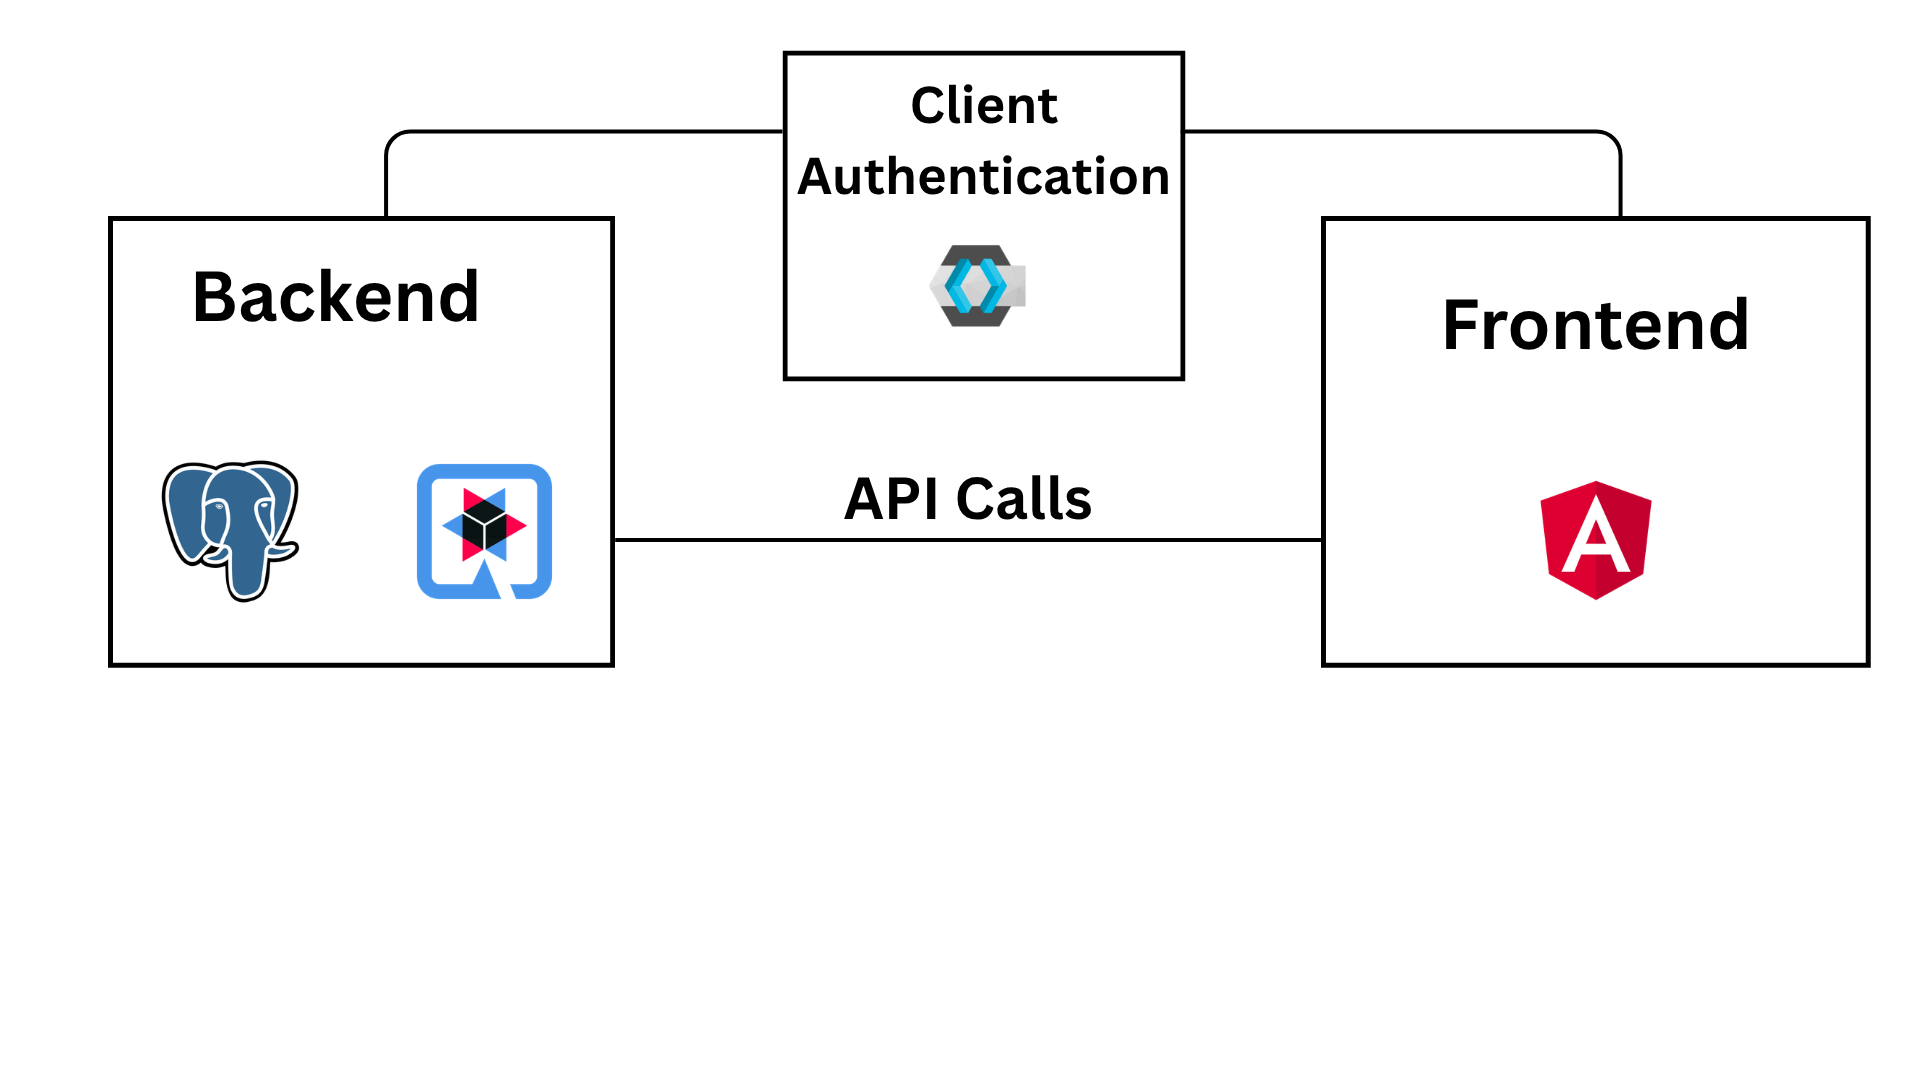
\includegraphics[width=1\textwidth, height=0.8\textheight, keepaspectratio]{pics/Architecture.png}
    \caption{Erstes Entity-Relationship-Diagramm der Anwendung}
    \label{fig:erd_v1}
\end{figure}



\subsection{Herausforderungen im Entwicklungsprozess}

Im Verlauf der Diplomarbeit traten mehrere strukturelle Herausforderungen auf, die
im Sinne einer transparenten Dokumentation offen dargestellt werden sollen.

Zu Beginn der Implementierungsphase wurde ohne vollständig ausgearbeitetes
Gesamtkonzept mit der Programmierung begonnen. Das Entity-Relationship-Diagramm
wurde parallel zur Entwicklung erstellt, wodurch sich die Datenbankstruktur
dynamisch entwickelte. Dieses iterative Vorgehen führte zwar zu schneller
praktischer Umsetzung, hatte jedoch den Nachteil, dass strukturelle Änderungen
im Nachhinein größeren Anpassungsaufwand verursachten.

\begin{figure}[h]
    \centering
    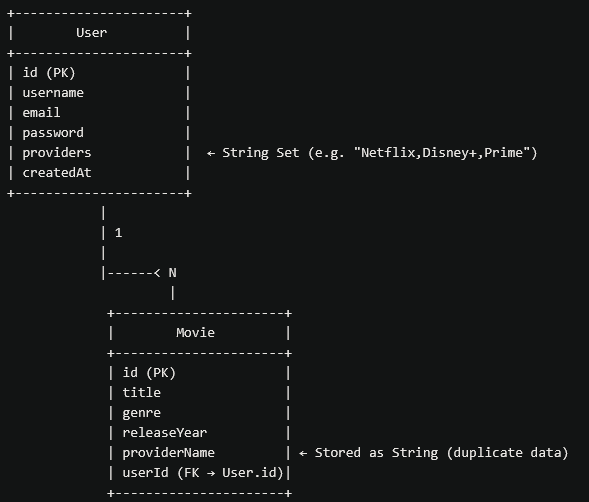
\includegraphics[width=0.9\textwidth]{pics/erd_v1}
    \caption{Erstes Entity-Relationship-Diagramm der Anwendung}
    \label{fig:erd_v1}
\end{figure}

Eine weitere wesentliche Herausforderung ergab sich durch die späte Integration
von Keycloak als Identity- und Access-Management-Lösung. Ursprünglich war die
Benutzerverwaltung eigenständig implementiert worden. Durch die nachträgliche
Einführung von Keycloak mussten die bestehenden User-Strukturen grundlegend
überarbeitet werden. Dies hatte zur Folge, dass die Benutzerentitäten angepasst
werden mussten, die Authentifizierungs- und Autorisierungslogik neu strukturiert
wurde sowie abhängige Klassen und Beziehungen refaktoriert und teilweise neu
implementiert werden mussten. Diese Umstellung führte zu zusätzlichem
Entwicklungsaufwand, zeigte jedoch zugleich die Bedeutung einer frühzeitigen
Architekturentscheidung -- insbesondere im Bereich der Sicherheits- und
Authentifizierungsmechanismen.

\begin{figure}[h]
    \centering
    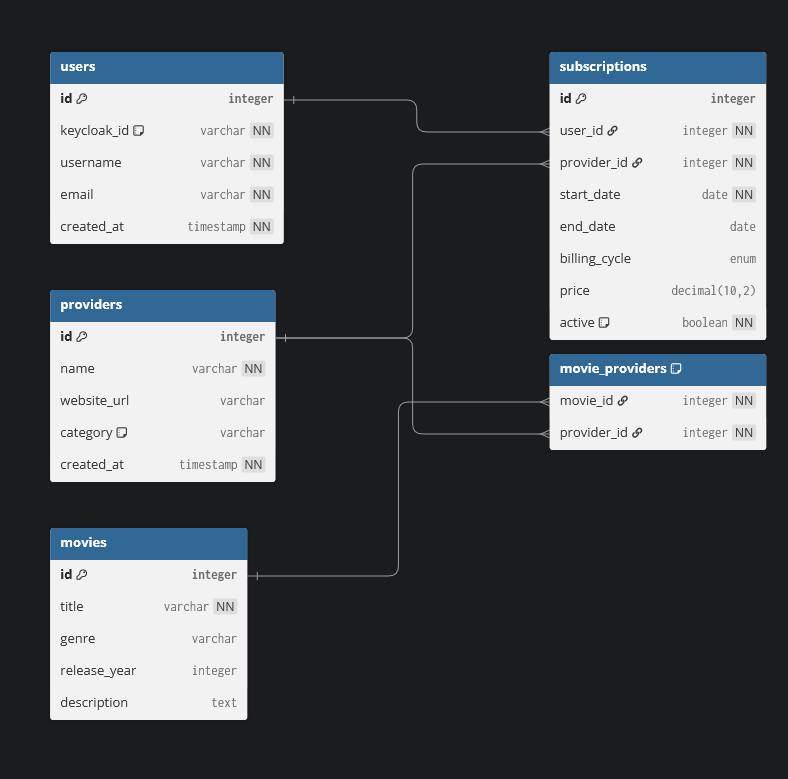
\includegraphics[width=0.9\textwidth]{pics/erd_v2}
    \caption{Überarbeitetes Entity-Relationship-Diagramm nach Integration von Keycloak}
    \label{fig:erd_v2}
\end{figure}


\subsection{Modellierung der Many-to-Many-Beziehung und strukturelle Weiterentwicklung}

Im weiteren Verlauf der Systemarchitektur zeigte sich deutlich der Mehrwert einer
sauberen relationalen Modellierung, insbesondere bei der Abbildung von
Many-to-Many-Beziehungen.

Im Kontext der vorliegenden Applikation -- einem Mediatheken-Abonnement-Manager --
besteht zwischen den Entitäten \textit{User} und \textit{Provider} keine einfache
1:n-Beziehung, sondern eine n:m-Beziehung. Ein Benutzer kann mehrere Anbieter
abonnieren, während ein Anbieter von mehreren Benutzern genutzt werden kann.

Die Einführung einer eigenständigen Relationstabelle (\texttt{UserProviderSubscription})
dient hierbei nicht ausschließlich der technischen Verknüpfung zweier Fremdschlüssel.
Vielmehr übernimmt diese Tabelle eine fachlich zentrale Rolle innerhalb des
Domänenmodells. In der Relationstabelle werden zusätzliche Attribute gespeichert,
die die konkrete Ausprägung der Beziehung beschreiben:

\begin{itemize}
    \item Beginn des Abonnements (Startdatum)
    \item Ende des Abonnements (Enddatum)
    \item Zahlungszyklus (Enum: monatlich oder jährlich)
\end{itemize}

Diese Attribute gehören semantisch weder ausschließlich zum Benutzer noch
ausschließlich zum Anbieter, sondern definieren die konkrete Vertragsbeziehung
zwischen beiden Entitäten. Die Modellierung über eine separate Relationstabelle
ermöglicht somit eine fachlich korrekte Abbildung der Geschäftslogik, die
Erweiterbarkeit um weitere beziehungsbezogene Attribute -- etwa Preis, Rabatt
oder Kündigungsstatus -- sowie eine klare Trennung der Verantwortlichkeiten
innerhalb des Datenmodells. Gerade an dieser Stelle wird deutlich, dass
relationale Datenbanken ihre Stärke bei strukturierten und stark
beziehungsorientierten Datenmodellen ausspielen.

\subsection{Reflexion der anfänglichen Modellierungsentscheidung}

Rückblickend stellt sich die anfängliche Entscheidung, Anbieter als
\texttt{Set<String>} direkt innerhalb der User-Entität zu speichern, als
struktureller Fehler heraus. Diese vereinfachte Modellierung war zwar für einen
ersten Prototyp funktional ausreichend, führte jedoch zu mehreren konzeptionellen
Einschränkungen:

\begin{enumerate}
    \item Es konnten keine anbieterspezifischen Metadaten gespeichert werden
    (z.\,B. Website, Kategorie oder Beschreibung).
    \item Die konkrete Ausgestaltung der Beziehung -- Startdatum, Zahlungszyklus
    etc. -- war nicht modellierbar.
    \item Eine konsistente Datenhaltung war nicht gewährleistet, da String-Werte
    fehleranfällig und nicht referenziell abgesichert sind.
    \item Erweiterungen des Systems hätten tiefgreifende strukturelle Änderungen
    erfordert.
\end{enumerate}

Insbesondere der Umstand, dass beziehungsrelevante Informationen nicht abgebildet
werden konnten, verdeutlicht die Problematik dieser frühen Designentscheidung.
Die Speicherung als String-Set widersprach den Grundprinzipien der Normalisierung
und verhinderte eine skalierbare Weiterentwicklung des Systems. Erst durch die
Einführung einer eigenständigen \texttt{Provider}-Entität sowie einer
Relationstabelle konnte das Datenmodell den fachlichen Anforderungen der
Applikation gerecht werden. Diese Umstrukturierung stellt einen wesentlichen
architektonischen Reifeprozess im Projektverlauf dar.


\begin{spacing}{1}
\chapter{Gemeinsame Architektur}\label{chapter:connectedArchitecture}  % <-- Titel + label geändert
\end{spacing}
% ============================================================
% GEMEINSAME ARCHITEKTUR-SECTION
% Empfehlung: In deiner architecture.tex oder als eigenes
% Kapitel vor den technischen Einzelteilen
% ============================================================

\section{Gesamtarchitektur der Anwendung}
\setauthor{Markus Tran}

Die vorliegende Anwendung folgt einer klar getrennten Client-Server-Architektur,
bei der Frontend und Backend als eigenständige Einheiten entwickelt wurden und
ausschließlich über definierte REST-Schnittstellen miteinander kommunizieren.

Das Frontend wurde von \textit{Abdulkerim Cufurovic} als Single-Page-Application
mit Angular umgesetzt und übernimmt die gesamte Darstellung, Navigation und
Benutzerinteraktion. Das Backend, dessen Implementierung Gegenstand des vorliegenden
Teils der Diplomarbeit ist, wurde mit Quarkus realisiert und stellt die
Geschäftslogik, Datenbankanbindung sowie die Kommunikation mit der externen
TMDB API bereit.

Die Authentifizierung beider Schichten erfolgt über Keycloak als zentralen
Identity-Provider. Dieses Zusammenspiel ist in Abbildung~\ref{fig:gesamtarchitektur}
dargestellt.

\begin{figure}[h]
    \centering
    \includegraphics[width=0.95\textwidth]{images/architektur_gesamt}
    \caption{Gesamtarchitektur der Anwendung mit Frontend, Backend und Keycloak}
    \label{fig:gesamtarchitektur}
\end{figure}

Die strikte Trennung zwischen Frontend und Backend bietet mehrere Vorteile.
Beide Schichten können unabhängig voneinander weiterentwickelt, getestet und
deployed werden. Änderungen an der Benutzeroberfläche erfordern keine Anpassungen
im Backend und umgekehrt, solange die vereinbarten Schnittstellen eingehalten
werden. Diese Architekturentscheidung war für die Aufteilung der Diplomarbeit
in zwei eigenständige Projektteile grundlegend.

\newpage
\pagenumbering{Roman}
\setcounter{page}{\value{RPages}}
\input{glossary}
\glsnogroupskiptrue
\IfStrEq{\thesislang}{de}
{
    \printglossary[title=Glossar,toctitle=Glossar]
}
{
    \printglossary[title=Glossary,toctitle=Glossary]
}
\spacing{1}{
\IfStrEq{\thesislang}{de}
{
    \bibliographystyle{ieeetrande}
}
{
    \bibliographystyle{IEEEtran}
}
\bibliography{bib}
}
\listoffigures
\listoftables
\lstlistoflistings
\appendix
\addchap{Anhang}
\input{./sections/appendix}

\end{document}